\chapter{Problema}
\label{sec:problema}

All'interno di questo capitolo sarà esposto il problema che si intende affrontare, ovvero la creazione di un marketplace decentralizzato basato su blockchain per la vendita sicura e trasparente di asset di vario genere.

I marketplace centralizzati sono molto diffusi, ma ad oggi presentano diverse criticità. Un'importante criticità è la richiesta di una fiducia spropositata verso l'entità centrale. Un utente, infatti, deve affidare diversi dati personali e sensibili per poter usufruire del servizio offerto. Inoltre, le transazioni vengono gestite centralmente, rendendole non trasparenti e soggette a manipolazioni. In figura \ref{fig:defivscefi} è possibile visualizzare come un sistema centralizzato è basato su una singola entità, mentre un sistema decentralizzato è composto da una rete di partecipanti che collaborano tra loro.  

\begin{figure}[H]
    \centering
    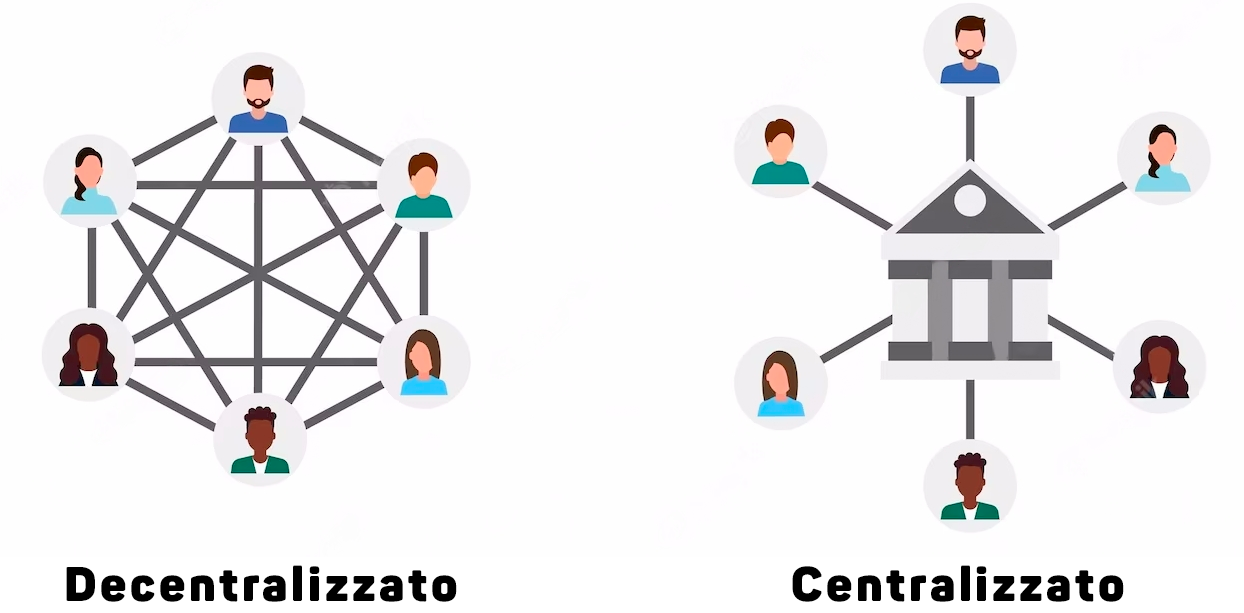
\includegraphics[width=0.79\textwidth]{images/DEFIvsCEFI.png}
    \caption{Differenza tra centralizzato e decentralizzato}
    \label{fig:defivscefi}
\end{figure}

Sono molteplici le ragioni che rendono necessario un nuovo modello di business, in grado di fornire un ambiente consono alle esigenze di venditori e acquirenti senza la necessità di un intermediario. 

Questo progetto si propone di risolvere il problema presentato, creando un marketplace decentralizzato basato su blockchain.